\documentclass[11pt]{article}
%\usepackage{graphicx}
\usepackage{booktabs}
\usepackage[backend=bibtex]{biblatex}
%\addbibresource{myBibRefsFile.bib}
%\usepackage[backend=bibtex,style=verbose-trad2]{biblatex}
\bibliography{IT.bib}
\usepackage{float}

%\usepackage[margin=1in]{geometry}
\usepackage{fancyhdr}
%\pagestyle{fancy}
\usepackage{amsmath}
%\usepackage{amssymb}
%\usepackage[table]{xcolor}
\usepackage{bm}
\usepackage{array}
\usepackage{mathtools}
\usepackage{soul,soulutf8}
\usepackage{url,color}
\usepackage{fullpage}
\usepackage[english]{babel}

\usepackage[utf8]{inputenc}
\lhead{STA 4001: Stochastic Processes}
\chead{}
\rhead{\textup{CUHK(SZ) Fall 2018}}


\usepackage{amsmath,amsthm,amssymb}
%\usepackage{extarrows}
%\usepackage{breqn}
\usepackage{mathtools}
\DeclarePairedDelimiter\ceil{\lceil}{\rceil}
\DeclarePairedDelimiter\floor{\lfloor}{\rfloor}
\newcommand{\N}{\mathbb{N}}
\newcommand{\Z}{\mathbb{Z}}
\newcommand{\trans}{^{\mathrm T}}

\newenvironment{theorem}[2][Theorem]{\begin{trivlist}
\item[\hskip \labelsep {\bfseries #1}\hskip \labelsep {\bfseries #2.}]}{\end{trivlist}}
\newenvironment{lemma}[2][Lemma]{\begin{trivlist}
\item[\hskip \labelsep {\bfseries #1}\hskip \labelsep {\bfseries #2.}]}{\end{trivlist}}
\newenvironment{exercise}[2][Exercise]{\begin{trivlist}
\item[\hskip \labelsep {\bfseries #1}\hskip \labelsep {\bfseries #2.}]}{\end{trivlist}}
\newenvironment{reflection}[2][Reflection]{\begin{trivlist}
\item[\hskip \labelsep {\bfseries #1}\hskip \labelsep {\bfseries #2.}]}{\end{trivlist}}
\newenvironment{proposition}[2][Proposition]{\begin{trivlist}
\item[\hskip \labelsep {\bfseries #1}\hskip \labelsep {\bfseries #2.}]}{\end{trivlist}}
\newenvironment{corollary}[2][Corollary]{\begin{trivlist}
\item[\hskip \labelsep {\bfseries #1}\hskip \labelsep {\bfseries #2.}]}{\end{trivlist}}
\DeclareMathOperator{\tr}{tr}
\DeclareMathOperator{\rank}{rank}
\DeclareMathOperator{\Span}{span}
\DeclareMathOperator{\row}{row}
\DeclareMathOperator{\col}{col}
\DeclareMathOperator{\range}{range}
\DeclareMathOperator{\Null}{Null}
\DeclarePairedDelimiterX{\inp}[2]{\langle}{\rangle}{#1, #2}
\DeclareMathOperator{\Proj}{Proj}
\newcommand{\diff}{\,\mathrm{d}}
\DeclareMathOperator{\trace}{trace}
\newcommand{\Her}{^{\mathrm H}}
\DeclareMathOperator{\diag}{diag}
\newcommand{\Var}{\mathrm{Var}}
%\usepackage{listings}
%\usepackage{color} %red, green, blue, yellow, cyan, magenta, black, white
%\definecolor{mygreen}{RGB}{28,172,0} % color values Red, Green, Blue
%\definecolor{mylilas}{RGB}{170,55,241}
%
%
%\lstset{language=Matlab,%
%    %basicstyle=\color{red},
%    breaklines=true,%
%    morekeywords={matlab2tikz},
%    keywordstyle=\color{blue},%
%    morekeywords=[2]{1}, keywordstyle=[2]{\color{black}},
%    identifierstyle=\color{black},%
%    stringstyle=\color{mylilas},
%    commentstyle=\color{mygreen},%
%    showstringspaces=false,%without this there will be a symbol in the places where there is a space
%    numbers=left,%
%    numberstyle={\tiny \color{black}},% size of the numbers
%    numbersep=9pt, % this defines how far the numbers are from the text
%    emph=[1]{for,end,break},emphstyle=[1]\color{red}, %some words to emphasise
%    %emph=[2]{word1,word2}, emphstyle=[2]{style},    
%}
\usepackage{listings}
\RequirePackage{listings}
\RequirePackage{xcolor}
\definecolor{dkgreen}{rgb}{0,0.6,0}
\definecolor{gray}{rgb}{0.5,0.5,0.5}
\definecolor{mauve}{rgb}{0.58,0,0.82}
\lstset{
  frame=tb,
  aboveskip=3mm,
  belowskip=3mm,
  showstringspaces=false,
  columns=flexible,
  framerule=1pt,
  rulecolor=\color{gray!35},
  backgroundcolor=\color{gray!5},
  basicstyle={\small\ttfamily},
  numbers=none,
  numberstyle=\tiny\color{gray},
  keywordstyle=\color{blue},
  commentstyle=\color{dkgreen},
  stringstyle=\color{mauve},
  breaklines=true,
  breakatwhitespace=true,
  tabsize=3,
}

\newcommand{\degree}{\ensuremath{^\circ}}
\begin{document}
\title{\bfseries\upshape{Solution to Assignment 4}}%replace X with the appropriate number
\author{\textit{I will appreciate it if you could give me some advice on my assignment!}} %if necessary, replace with your course title
\maketitle
\section*{phd exercises}
\begin{enumerate}
\item
Suppose that $D^0$ is \emph{symmetric} and we apply \textbf{SR1} method to solve the positive definite quadratic problem $f(x)=\frac{1}{2}x\trans Qx-b\trans x$, i.e., $D^k$ is updated according to the formula
\begin{equation}\label{Eq:7}
D^{k+1} = D^k+\frac{(y^k)(y^k)\trans}{\inp{q^k}{y^k}},
\end{equation}
where $y^k = p^k - D^kq^k$. 
\begin{enumerate}
\item
Show that we have 
\begin{equation}
\begin{array}{ll}
D^{k+1}q^i=p^i,
&
\mbox{for all $k$ and $i\le k$},
\end{array}\label{Eq:1}
\end{equation}
\item
Conclude that for a positive definte quadratic problem, after $n$ steps for which $n$ linearly independent increments $q^0,q^1,\dots,q^{n-1}$ are obtained, $D^n$ is equal to the \emph{inverse Hessian} of the cost function.
\end{enumerate}
\begin{proof}

Notations:
\begin{itemize}
\item
$D^k$: Approximation of the inverse of Hessain matrix $[\nabla^2f(x^k)]^{-1}$ at $k$th iteration
\item
$p^k$: difference between argument at $k$th iteration, i.e., $p^k = x^{k+1} - x^k$
\item
$q^k$: difference between gradient of function at $k$th iteration, i.e., $q^k=\nabla f(x^{k+1}) - \nabla f(x^k)$
\end{itemize}
\begin{enumerate}
\item
We apply induction on $k$ to show this formula.
\begin{itemize}
\item
As $k=0$, as the \emph{secant equation} (2.43) in the textbook has to be satsified, i.e.,
\[
D^{k+1}(\nabla f^{k+1} - \nabla f^k)= x^{k+1} - x^k,
\]
and thus taking $k=0$ we obtain the desired formula $D^1q^0=p^0$.
\item
Then we assume (\ref{Eq:1}) holds for some value $k>1$, and show that it also holds for $k+1$. (i.e., given $D^{k+1}q^i = p^i$ with $i\le k$, we aim to show $D^{k+2}q^{i} = p^{i}$ with $i\le k+1$) 
\begin{enumerate}
\item[(i)]
First consider the term $\inp{p^{k+1}-D^{k+1}q^{k+1}}{q^i}$ for $i\le k$:
\begin{align}
\inp{p^{k+1}-D^{k+1}q^{k+1}}{q^i}&=
\inp{p^{k+1}}{q^i}- 
\inp{q^{k+1}}{(D^{k+1})\trans q^i}\\
&=\inp{p^{k+1}}{q^i}- 
\inp{q^{k+1}}{D^{k+1} q^i}\\
&=\inp{p^{k+1}}{q^i}- \inp{q^{k+1}}{p^i}\label{Eq:4}\\
&=\inp{p^{k+1}}{Qp^i}- \inp{Qp^{k+1}}{p^i}\label{Eq:5}\\
&=0,
\end{align}
where (\ref{Eq:4}) is obtained by applying the hypothesis $D^{k+1}q^i=p^i$; and (\ref{Eq:5}) is obtained by computing the formula $q^j=\nabla f(x^{j+1}) - \nabla f(x^{j}) = Qx^{j+1} - Qx^{j}=Q(x^{j+1}-x^j)=Qp^j$.
\item[(ii)]
Thus we can derive the formula for $D^{k+2}q^i:$
\begin{align}
D^{k+2}q^i&=D^{k+1}q^i+\frac{(y^{k+1})(y^{k+1})\trans}{\inp{q^{k+1}}{y^{k+1}}}q^i\label{Eq:8}\\
&=D^{k+1}q^i+\frac{y^{k+1}\inp{y^{k+1}}{q^i}}{\inp{q^{k+1}}{y^{k+1}}}\\
&=D^{k+1}q^i+\frac{y^{k+1}\inp{p^{k+1} - D^{k+1}q^{k+1}}{q^i}}{\inp{q^{k+1}}{y^{k+1}}}\label{Eq:10}\\
&=0,\label{Eq:11}
\end{align}
where (\ref{Eq:8}) is due to the update formula (\ref{Eq:7}); (\ref{Eq:10}) is due to the formula $y^k=p^k-D^kq^k$; (\ref{Eq:11}) is due to the formula in (i)
\end{enumerate}
Combining (i) and (ii), the proof in (a) is complete.
\end{itemize}
\item
If this algorithm is performed $n$ steps and $q^0,\dots,q^{n-1}$ are linearly independent, taking $k=n-1$ at (\ref{Eq:1}),
\begin{equation}\label{Eq:12}
\begin{array}{ll}
p^i = D^{n}q^i=D^{n}Qp^i,
&
i=0,1,\dots,n-1
\end{array}
\end{equation}
Note that here $Q:=H$ is the Hessian matrix of the cost function. Thus we re-write (\ref{Eq:12}) as:
\[
D^nQP=P\Longleftrightarrow
(D^nQ-I)P=0,
\]
where $P:=\begin{pmatrix}
(p^0)\trans&(p^1)\trans&\cdots&(p^{n-1})\trans
\end{pmatrix}\trans$ is nonsingular due to the linear independence of $q^{j}$'s and $p^j=Q^{-1}q^j$ for $j=0,\dots,n-1$. It follows that
\[
D^nQ-I=0\implies D^n=Q^{-1},
\]
i.e., $D^n$ is equal to the \emph{inverse Hessian} of the cost function.
\end{enumerate}
\end{proof}
\end{enumerate}
\clearpage
\section*{Project 1:
Gauss-Newton Method for Truncated SVD}

\subsection*{A copy of my Code}
\begin{lstlisting}[language=matlab]
function [X, iter] = myGN(A,X0,tol,maxiter)
% Input:
%        A: given matrix
%       X0: initial guess
%      tol: tolerance
%  maxiter: maximum iterations
%Output:
%        X: solution to the opt
%     iter: number of iterations

k = size(X0,2);
I = speye(k);
for iter = 1:maxiter
    M = X0'*X0;
    Y = X0/M;
    Z = A*Y;
    X = Z - X0 * ((Y'*Z-I)/2);
    if norm(X - X0,'fro')^2 <= tol^2 * trace(M),break;end
    X0 = X;
end
end
\end{lstlisting}
\subsection*{Matlab screen printout}
\begin{figure}[H]
\centering
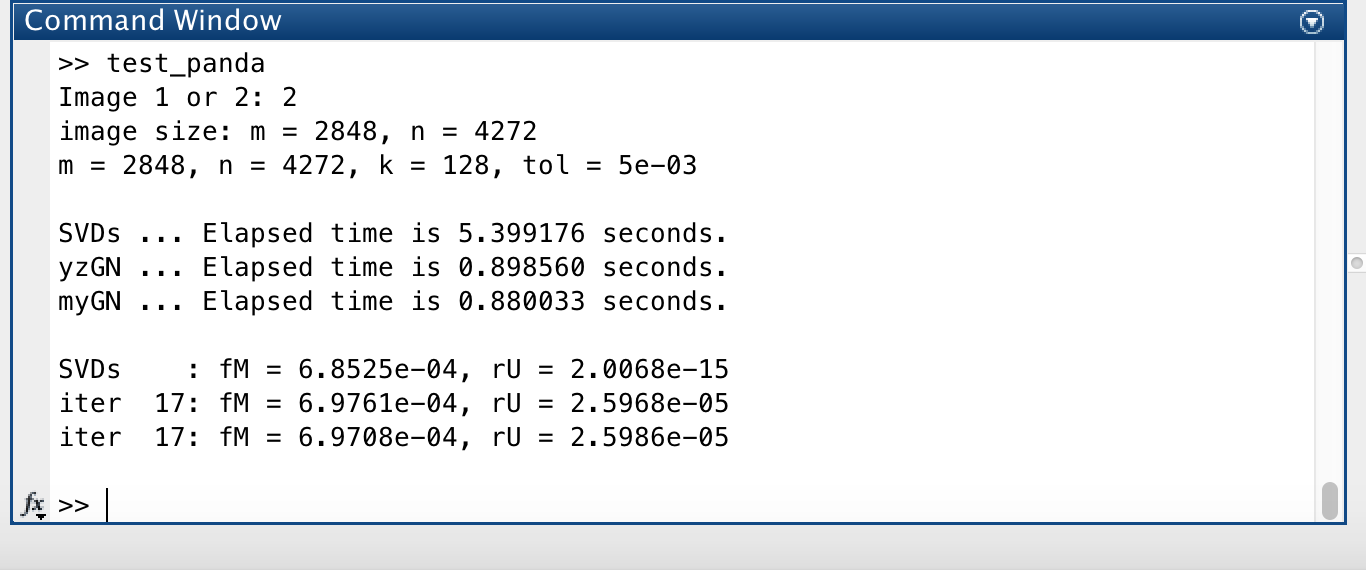
\includegraphics[width=16cm]{f_1.png}
\caption{Matlab screen printout from Image $\#$2}
\end{figure}
\clearpage
\subsection*{Figure generated from run 2}
\begin{figure}[H]
\centering
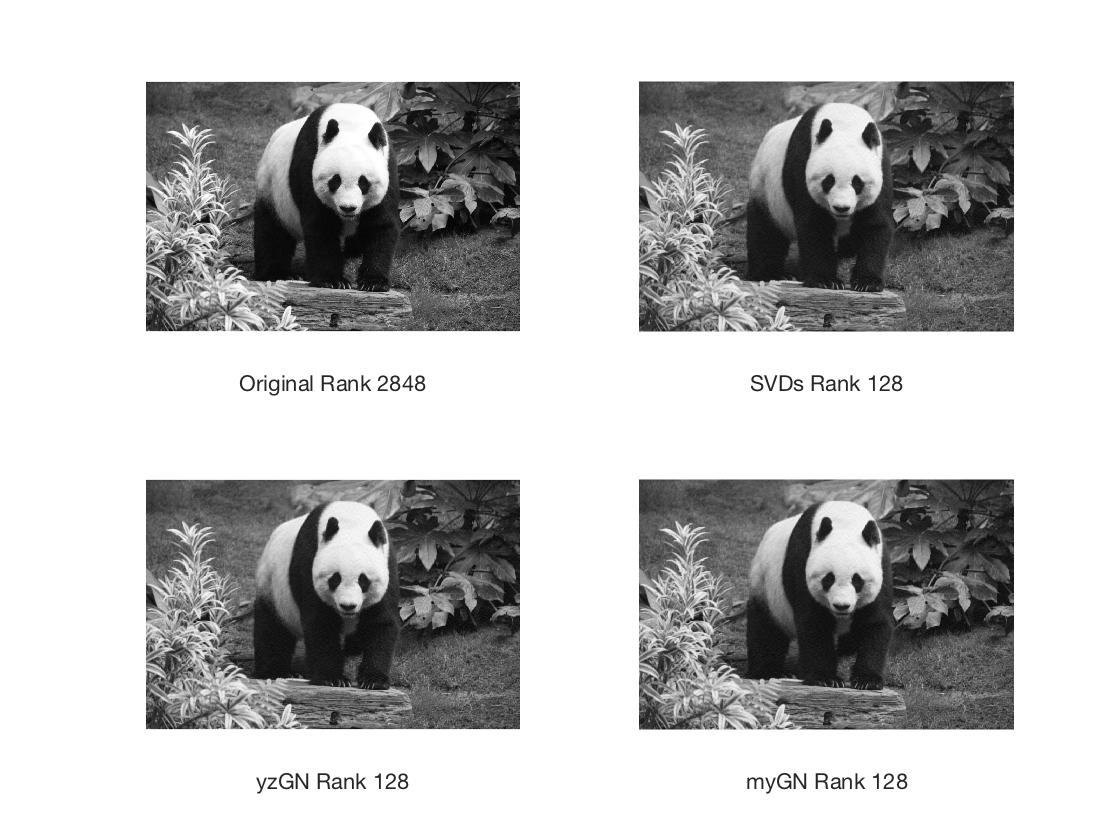
\includegraphics[width=16cm]{f_2}
\caption{Figure generated from Image $\#$2}
\end{figure}
\clearpage
\subsection*{A short summary}
\paragraph{Introduction}
This project aims to apply Gauss-Newton method to compute a symmetric rank product $XX\trans$ that is closest to $A$ in Frobenius norm. The process is just two-line MATLAB code:
\begin{align*}
Y&\leftarrow X^k((X^k)\trans X^k)^{-1}\\
X^{k+1}&\leftarrow AY - X^k(Y\trans AY - I)/2
\end{align*}
Although the process is simple, we still need to care about the arrangement of computation, otherwise our code will have long and unnecessary computing time.
\paragraph{Do Avoid repeated computation}
\begin{enumerate}
\item
For example, the update of $X^{k+1}$ requires twice computation of $AY$, so it's better to compute this value and save it using a new variable.
\item
Another example is that the stopping criteria requires the value of $\mbox{norm(X)}$, i.e., $\sqrt{\trace(X\trans X)}$, and the update for $Y$ also requires the computation of $X\trans X$, so we should compute this value in advance and save it using a new variable. 
\item
Moreover, computing $X * [(Y\trans AY - I)/2]$ is faster than computing $[X(Y\trans AY - I)]/2$, since the former only requires the division operation on a smaller size matrix.
\end{enumerate} 
\paragraph{Save necessity before iteration}
The update of $X$ requires the call of large scale identity for each iteration, which is time-consuming. So we should save the identiy matrix in sparse form \emph{before} iteration.










\clearpage




\section*{Project 2:
Solving LP Barrier Systems by Newton’s Method}
\subsection*{Deviations}
The Newton's method  to the Barrier system gives:
\[
\begin{pmatrix}
x^{k+1}\\y^{k+1}\\z^{k+1}
\end{pmatrix}
=
\begin{pmatrix}
x^{k}\\y^{k}\\z^{k}
\end{pmatrix}
-
[F'_{\mu}(x,y,z)]^{-1}F_{\mu}\implies
\begin{pmatrix}
dx\\dy\\dz
\end{pmatrix}=
-[F'_{\mu}(x,y,z)]^{-1}F_{\mu}
\]
Leftmultiplying with $F'_{\mu}(x,y,z)$, we derive:
\[
F'_{\mu}(x,y,z)\begin{pmatrix}
dx\\dy\\dz
\end{pmatrix}
=
-F_\mu:=\begin{pmatrix}
r_d\\r_p\\r_c
\end{pmatrix}
\]
We set 
\begin{align*}
f_1:&=A\trans y+z-c\\
f_2:&=Ax-b\\
f_3:&=(x_1z_1-\mu,x_2z_2-\mu,\dots,x_nz_n-\mu)\trans
\end{align*}
\begin{itemize}
\item
Here we derive a concise expression for the \emph{Jacobian matrix} $F'_\mu(x,y,z)$. Note that
\begin{align*}
\nabla_x f_1&=0,\qquad
\nabla_yf_1=A,\qquad
\nabla_zf_1=I\\
\nabla_x f_2&=A\trans,\qquad
\nabla_yf_2=0,\qquad
\nabla_zf_2=0\\
\frac{\partial f_3(j)}{\partial x_j}&=z_j,\qquad
\frac{\partial f_3(j)}{\partial y_j}=0,\qquad
\frac{\partial f_3(j)}{\partial z_j}=x_j,
\end{align*}
Therefore, 
\begin{itemize}
\item
the Jacobian matrix for $f_3$ is 
\[
J_3=[\frac{\partial f(i)}{\partial x_j,y_j,z_j}]_{n\times(3n)}=
\begin{bmatrix}
Z&0&X
\end{bmatrix}
\]
with $Z:=\diag(z_1,\dots,z_n)$ and $X:=\diag(x_1,\dots,x_n)$.
\item
the Jacobian matrices for $f_1,f_2$ are:
\begin{align*}
J_1&=\begin{bmatrix}
\nabla_x\trans f_1&
\nabla_y\trans f_1&
\nabla_z\trans f_1&
\end{bmatrix}=\begin{pmatrix}
0&A\trans&I
\end{pmatrix}
\\
J_2&=\begin{bmatrix}
\nabla_x\trans f_2&
\nabla_y\trans f_2&
\nabla_z\trans f_2&
\end{bmatrix}=\begin{pmatrix}
A&0&0
\end{pmatrix}
\end{align*}
\item
The Jacobian matrix for $F_\mu(x,y,z)$ is given by:
\[
F'_\mu(x,y,z)=
\begin{pmatrix}
J_1\\J_2\\J_3
\end{pmatrix}=
\begin{pmatrix}
0&A\trans&I\\A&0&0\\Z&0&X
\end{pmatrix},
\]
where $Z:=\diag(z_1,\dots,z_n)$ and $X:=\diag(x_1,\dots,x_n)$.
\end{itemize}
\item
After rearranging, it suffices to solve the system
\[
\begin{pmatrix}
A\trans&I&0\\0&0&A\\0&X&Z
\end{pmatrix}\begin{pmatrix}
dy\\dz\\dx
\end{pmatrix}=\begin{pmatrix}
r_d\\r_p\\r_c
\end{pmatrix}
\]
Or we write it into \emph{augumented form} and solve it for $dy$ first:
\[
\left[
\begin{array}{@{}ccc|c@{}}
A\trans&I&0&r_d\\
0&0&A&r_p\\
0&X&Z&r_c
\end{array} \right]
\xLongrightarrow{\text{row 1 left-multiply $X$}}
\left[
\begin{array}{@{}ccc|c@{}}
X A\trans&X&0&Xr_d\\
0&0&A&r_p\\
0&X&Z&r_c
\end{array} \right]\xLongrightarrow{\text{Add row 3 into row 1}}
\]
\[
\left[
\begin{array}{@{}ccc|c@{}}
X A\trans&0&-Z&Xr_d-r_c\\
0&0&A&r_p\\
0&X&Z&r_c
\end{array} \right]
\xLongrightarrow{\text{row 1 divided by $Z$}}
\left[
\begin{array}{@{}ccc|c@{}}
\frac{X}{Z} A\trans&0&-I&\frac{Xr_d-r_c}{Z}\\
0&0&A&r_p\\
0&X&Z&r_c
\end{array} \right]
\xLongrightarrow{\text{row 1 leftmutliply by $A$}}
\]
\[
\left[
\begin{array}{@{}ccc|c@{}}
A\frac{X}{Z} A\trans&0&-A&A\frac{Xr_d-r_c}{Z}\\
0&0&A&r_p\\
0&X&Z&r_c
\end{array} \right]
\xLongrightarrow{\text{Add row 2 into row 1}}
\left[
\begin{array}{@{}ccc|c@{}}
A\frac{X}{Z} A\trans&0&0&A\frac{Xr_d-r_c}{Z}+r_p\\
0&0&A&r_p\\
0&X&Z&r_c
\end{array} \right]
\]
Hence, we derive a formula for solving $dy$:
\[
A\frac{X}{Z}A\trans dy=A\frac{Xr_d-r_c}{Z}+r_p
\]

Then we want to apply back substitution to solve for $dx$ and $dz$. Recall the formula above that $Xdz+Zdx=r_c$,
 and to solve $dx$, we apply Gaussian elimination again:
\[
\left[
\begin{array}{@{}ccc|c@{}}
A\trans&I&0&r_d\\
0&0&A&r_p\\
0&X&Z&r_c
\end{array} \right]
\xLongrightarrow{\text{Add row 1 leftmutliplying $-X$ into row 3}}
\left[
\begin{array}{@{}ccc|c@{}}
A\trans&I&0&r_d\\
0&0&A&r_p\\
-XA\trans &0&Z&r_c-Xr_d
\end{array} \right]
\]
Therefore,
\[
-XA\trans dy+Zdx=r_c-Xr_d
\]
In summary, we derive formulas for solving $dx,dy$ and $dx$:
\[
\left\{
\begin{aligned}
A\frac{X}{Z}A\trans dy&=A\frac{Xr_d-r_c}{Z}+r_p\\
-XA\trans dy+Zdx&=r_c-Xr_d\\
Xdz+Zdx&=r_c
\end{aligned}
\right.
\]
We solve the small linear system $dy$ only, and after solving these small systems, $dz,dx$ are recovered by backsubstitutions:
\[
\left\{
\begin{aligned}
dx&=[XA\trans dy+(r_c-Xr_d)]/Z\\
dz &= \frac{r_c-Zdx}{X}
\end{aligned}
\right.
\]
\end{itemize}

\clearpage
\subsection*{A Copy of my Code}
\begin{lstlisting}[language=matlab]
function [dx,dy,dz] = mylinsolve(A,rd,rp,rc,x,z)
% Usage: Solving LP Barrier Systems by Newton’s Method
% Input:
%       A: m * n matrix
%      rd: n * 1 vector
%      rp: m * 1 vector
%      rc: n * 1 vector
%       x: n * 1 vector
%       z: n * 1 vector
%Output:
%      dx: n * 1 vector
%      dy: m * 1 vector
%      dz: n * 1 vector
n = length(rd);
d = x./z;
B = A * sparse(1:n,1:n,d) * A';
t1 = -x.*rd + rc;
t2 = A * (-t1./z) + rp;
dy = B \ t2;
dx = (t1 + x.*(A'*dy))./z;
dz = (rc - z.*dx)./x;
end
\end{lstlisting}
\clearpage
\subsection*{MATLAB Screen Printout for $p=1$}
\begin{figure}[H]
\centering
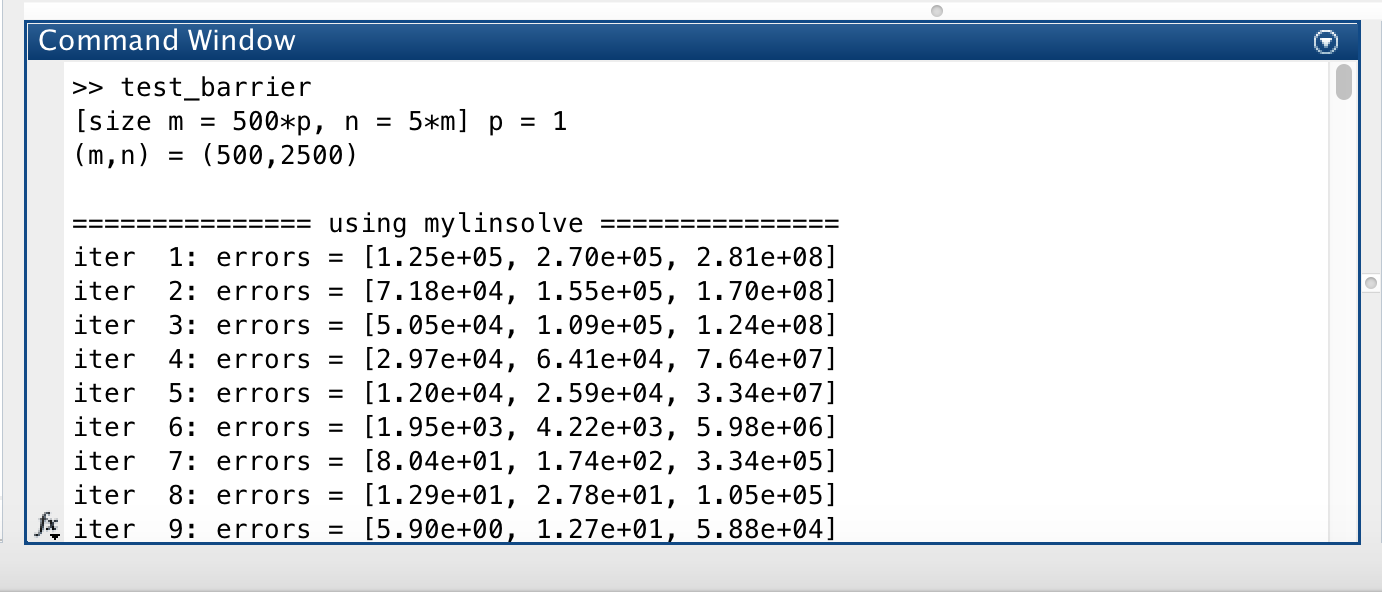
\includegraphics[width=16cm]{f_3}
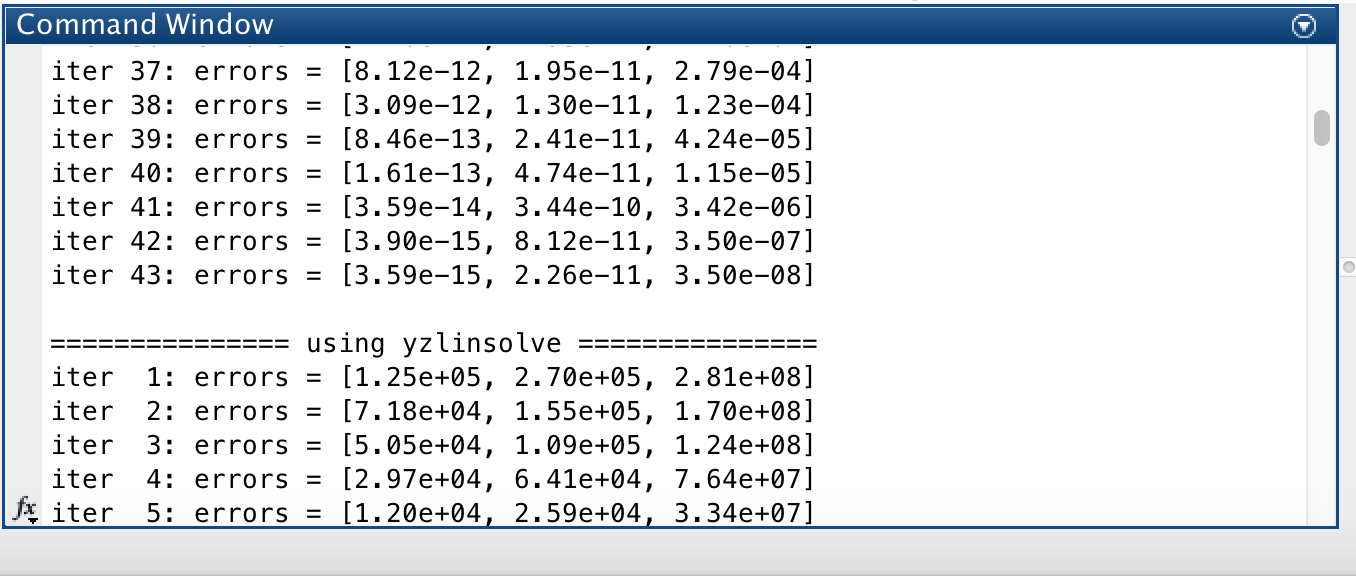
\includegraphics[width=16cm]{f_4}
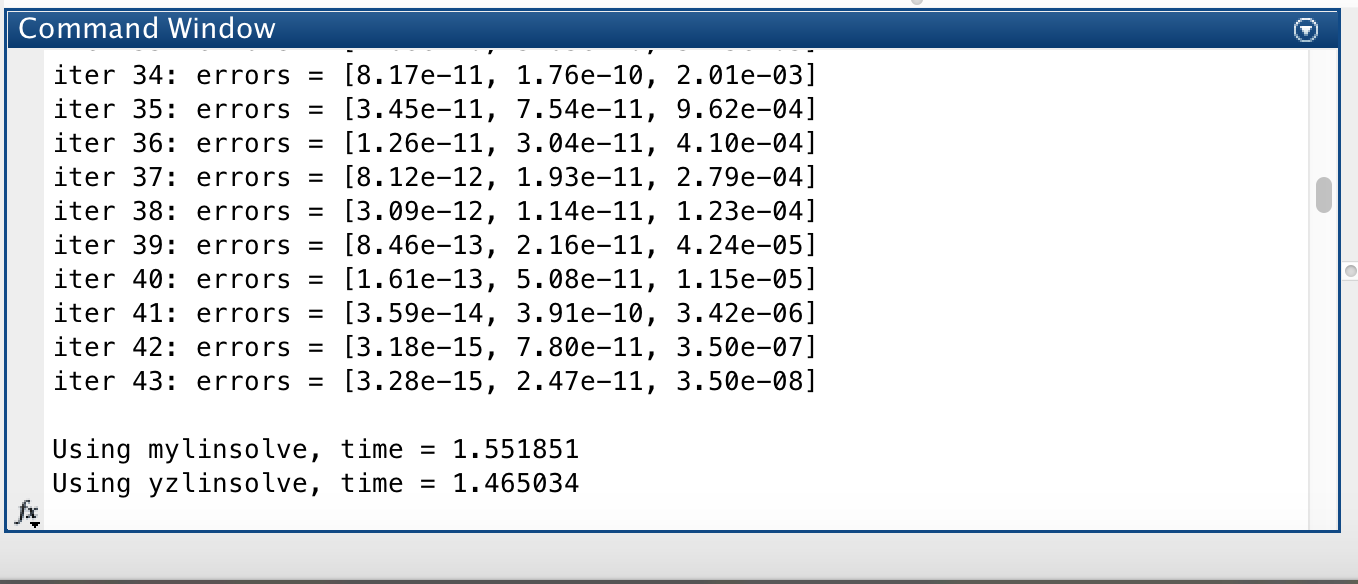
\includegraphics[width=16cm]{f_5}
\caption{MATLAB Screen Printout for $p=1$}
\end{figure}
\subsection*{MATLAB Screen Printout for $p=4$}
\begin{figure}[H]
\centering
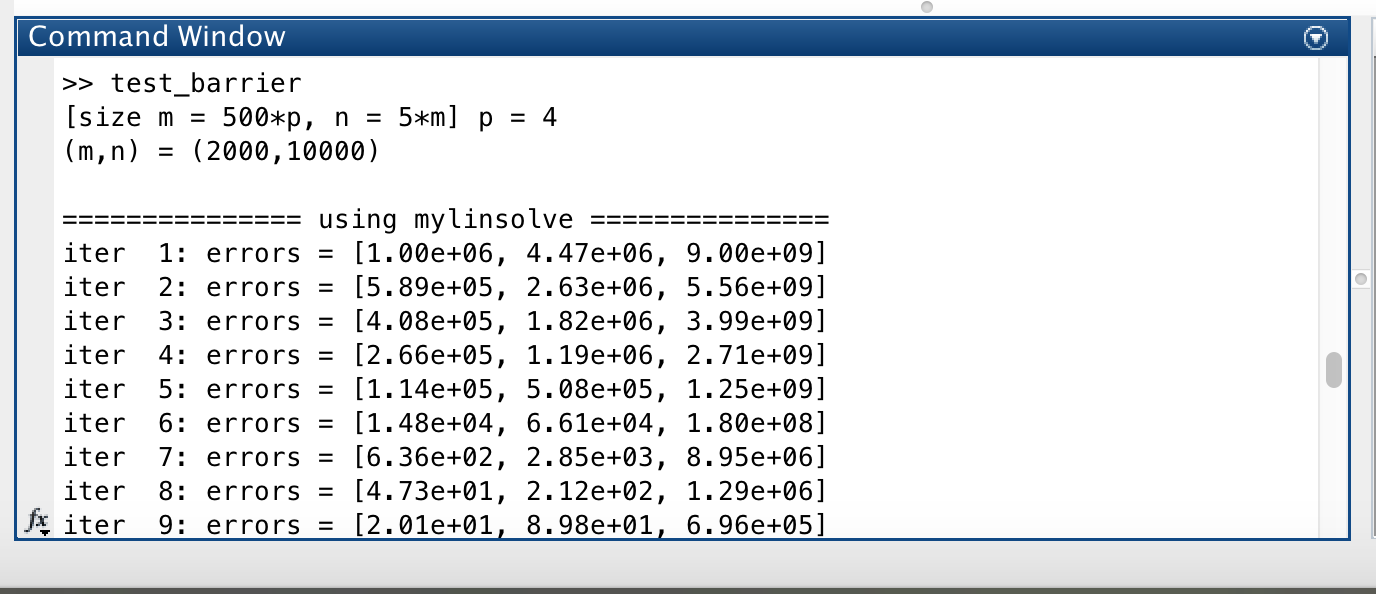
\includegraphics[width=16cm]{f_6}
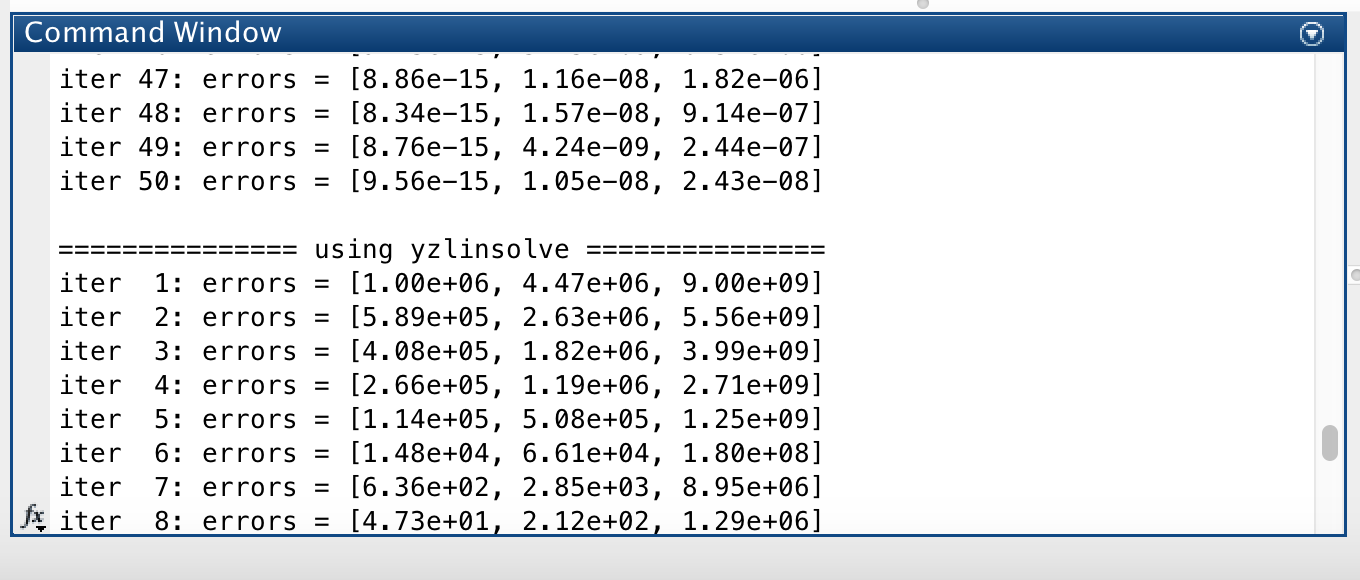
\includegraphics[width=16cm]{f_7}
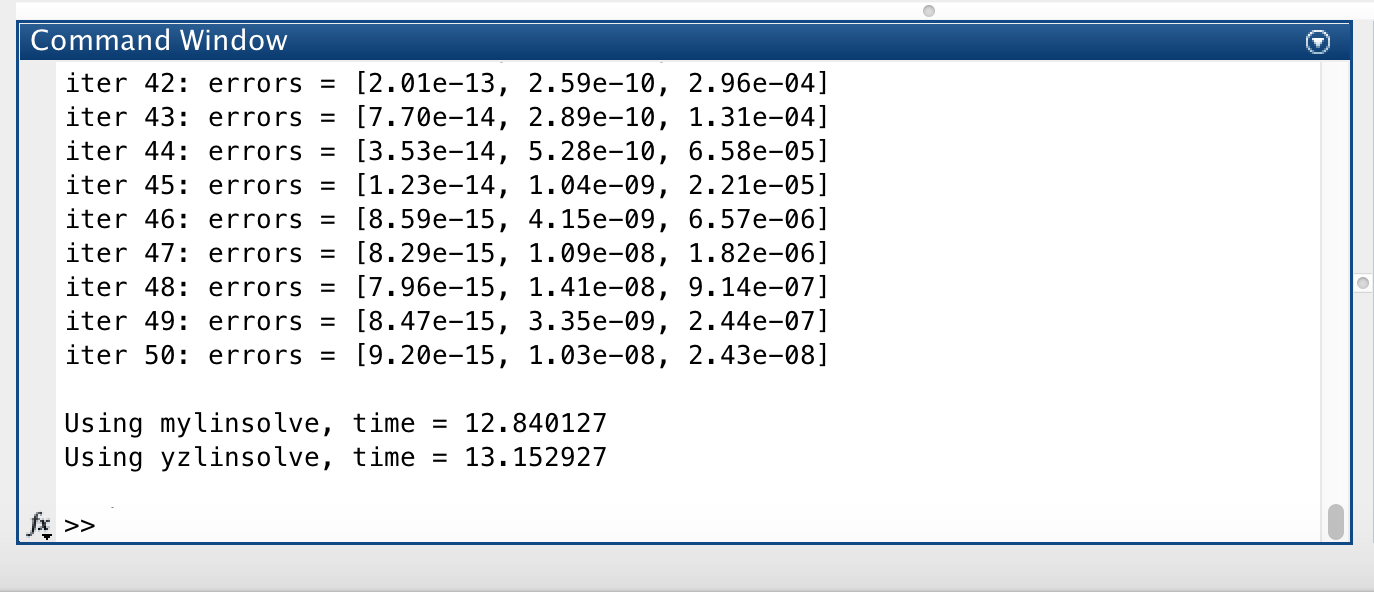
\includegraphics[width=16cm]{f_8}
\caption{MATLAB Screen Printout for $p=4$}
\end{figure}
\subsection*{A short summary}
\paragraph{Introduction}
This project aims to solve a LP Barrier Systems by Newton’s Method, i.e., applying Newton's method to solve linear systems.
\paragraph{Compute $dx$ and $dz$ Smartly}
During the computation, we need to solve a small linear system $dy$ first, after which we should not solve for $dz$ using the \emph{echelon echol form} directly, i.e., do not compute $dz=A^{-1}r_p$, which is computationally expansive. Instead, we derive the formula for $dx$ and $dz$ in terms of $dy$ sufficiently. The advantage is that we use the extra information for solving this system, and avoid some large-scale matrix inverse calculation processes. 
\paragraph{Appreciate the sparse form}
When computing the inverse of $A*\diag(d)*A'$, we should use the sparse form since the dimension for this matrix is large and most entries are zero.
\paragraph{Arrange Reasonable Computation}
For example, we need to use the balue $-x/*rd+rc$ for many times, so we can save it in advance and call them if necessary. Moreover, saving the matrix $\diag(x_1/z_1,\dots,x_n/z_n)$ is meaningless, since we can arrange computation such that it suffices to save the vector form $x./z$.












\end{document}